\documentclass[twoside]{article}

\usepackage[sc]{mathpazo} % Use the Palatino font
\usepackage[T1]{fontenc} % Use 8-bit encoding that has 256 glyphs
\linespread{1.05} % Line spacing - Palatino needs more space between lines
\usepackage{microtype} % Slightly tweak font spacing for aesthetics
\usepackage{color} % Permite cambiar el color del texto
%\usepackage{siunitx}
%\usepackage[twoside,width=16cm,height=24cm,left=3cm]{geometry}
\usepackage[hmarginratio=1:1,top=20mm,width=19cm,height=23cm,columnsep=15pt]{geometry} % Document margins
\usepackage{multicol} % Used for the two-column layout of the document
\usepackage[hang, small,labelfont=bf,up,textfont=it,up]{caption} % Custom captions under/above floats in tables or figures
\usepackage{booktabs} % Horizontal rules in tables
\usepackage{float} % Required for tables and figures in the multi-column environment - they need to be placed in specific locations with the [H] (e.g. \begin{table}[H])
\usepackage{hyperref} % For hyperlinks in the PDF

\usepackage[spanish]{babel}% idioma castellano
\usepackage[utf8]{inputenc}% esto es para poder poner los tildes directamente. Puede que cambie de versión a versión de sistema operativos (más información en http://www.aq.upm.es/Departamentos/Fisica/agmartin/webpublico/latex/FAQ-CervanTeX/FAQ-CervanTeX-6.html )
\usepackage{graphicx} % para insertar figuras
%\usepackage{subfigure} % para insertar figuras dentro de figuras
\usepackage{times} % plataforma
\usepackage{amsmath} % --para ecuaciones y algunos símbolos 
\usepackage{amssymb} % Libreria de Simbolos
\usepackage{enumerate} % Mas control en el uso de listas

\usepackage{bm}

\usepackage{lettrine} % The lettrine is the first enlarged letter at the beginning of the text
\usepackage{paralist} % Used for the compactitem environment which makes bullet points with less space between them

\usepackage{abstract} % Allows abstract customization
\renewcommand{\abstractnamefont}{\normalfont\bfseries} % Set the "Abstract" text to bold
\renewcommand{\abstracttextfont}{\normalfont\small\itshape} % Set the abstract itself to small italic text
\addto\captionsspanish{ % Modifica algunos nombres cambiandolos por los definidos a continuacion
        \def\contentsname{\'Indice}%
        \def\bibname{Referencias}%
        \def\tablename{Tabla}%
        \def\abstractname{Resumen}
        }

\usepackage{titlesec} % Allows customization of titles
\usepackage{fancyhdr} % Headers and footers
\pagestyle{fancy} % All pages have headers and footers
\fancyhead{} % Blank out the default header
\fancyfoot{} % Blank out the default footer
\fancyhead[C]{Laboratorio 6 $\bullet$ Cátedra Ledesma} % Custom header text
\fancyfoot[RO,LE]{\thepage} % Custom footer text
\newcommand{\grad}{$^{\circ}$}




\usepackage[utf8]{inputenc}  
\usepackage{amsmath}        
\usepackage{fullpage}       
\usepackage{booktabs}        
\usepackage{tikz}  
\usepackage[spanish]{babel}
\usepackage{pgfplots}        
\usepackage{float}            
\usepackage{hyperref}   
\usepackage{color}             
\usepackage{graphicx}        
\usepackage{xfrac}
\usepackage{titling}
\usepackage{amssymb}
\usepackage{multirow}
\hyphenpenalty=100000         
\pgfplotsset{compat=1.10}
\usepackage{subcaption}
\usepackage{natbib}
\usepackage{siunitx}
\sisetup{load-configurations = abbreviations}

\usepackage[format=plain,
            labelfont=it,
            textfont=it]{caption}

\usepackage{geometry}
\geometry{
left=20mm,
right=20mm,
}

\usepackage{multicol}

\begin{document}

\begin{titlepage}
\begin{center}

\textsc{\LARGE Laboratorio 7}\\[0.5cm]
\textsc{\Large Departamento de Física}\\[0.5cm]
\textsc{\Large Facultad de Ciencias Exactas y Naturales}\\[0.5cm]
\textsc{\Large Universidad de Buenos Aires}\\[1.5cm]

1er cuatrimestre 2021\\[1.5cm]

{ \huge \bfseries Aplicación del efecto Josephson a la generación de señales arbitrarias con aplicaciones a la metrología}\\[1.5cm]


%\begin{minipage}{0.8\textwidth}
%\begin{flushleft} \large


Alumno:
Pinto Zárate, José Daniel\\
\href{mailto:dann.2207@gmail.com}{dann.2207@gmail.com}

%\end{flushleft}
%\end{minipage}
\vfill
{\large \today}
\end{center}
\end{titlepage}


\begin{abstract}

El JAWS (Josephson Arbitrary Waveform Synthesizer) es un sintetizador de señales basado en el efecto Josephson. Cuando se conectan miles de junturas Josephson en serie, se puede aprovechar este efecto para generar señales arbitrarias. Para esto, se envían pulsos de corriente de alta frecuencia hacia esos arrays de junturas, sumergidas en Helio a 4.2K, y las mismas generan una tensión de salida que depende de constantes fundamentales, y por lo mismo tiene muy baja incertidumbre, del orden de los $1 \si{\volt}/10^10 \si{\volt}$. 
Existe un patrón específico de pulsos para cada señal que se quiera generar, y el mismo se obtiene mediante un algoritmo llamado modulación Sigma-Delta. En este trabajo se realizaron y comprobaron numéricamente distintos patrones de pulsos, generados mediante un algoritmo escrito siguiendo bibliografía especializada \cite{delarosa2011} \cite{aziz1996}

\end{abstract}

\begin{multicols}{2}


\section{Introducción}

\subsection{Efecto Josephson}

Los sistemas conocidos como Josephson Arbitrary Waveform Synthetizer (JAWS) \cite{behr2012} \cite{benz1996} \cite{benz1998} son sistemas basados en el efecto Josephson utilizados para la generación de formas de onda arbitrarias de tensión, en el cual la tensión generada depende de constantes fundamentales.

El efecto Josephson es un fenómeno que ocurre en junturas superconductoras separadas por una barrera muy delgada de algún material no superconductor al ser irradiadas por una frecuencia de microondas. En el caso del JAWS las junturas usadas son del tipo SNS (superconductor-normal-superconductor).



%como la constante de Planck, la carga eléctrica elemental y una frecuencia enlazada a relojes atómicos.

Estos sistemas utilizan arreglos, o {\it arrays}, de miles de junturas Josephson,  que son irradiadas por un tren de pulsos de corriente de tiempo corto, del orden de los GHz, con un patrón de repetición determinado por el tipo de señal que se quiere obtener. La tensión en una juntura está dada por:

\begin{equation}
    V_J = n \frac{h}{2e}f = n \Phi_0 f
    \label{eq:josephson}
\end{equation}

donde $h$ es la constante de Plank, $e$ la carga eléctrica elemental, $\Phi_0$ es el cuanto de flujo magnético, $n$ un número entero y $f$ la frecuencia de trabajo, en nuestro caso referida a un reloj atómico. Los pulsos que usaremos son binarios, lo que significa que los valores de $n$ posibles son $n=\pm 1$.

Cuando se conecta un número grande de junturas Josephson en serie, el efecto descrito en la ecuación \ref{eq:josephson} se suma por cada una de las junturas presentes, dando lugar a la posibilidad de generar voltajes ordenes de magnitud mayores a los de la juntura simple. 

El chip mostrado en la figura \ref{fig:chipJaws}, el que se va a utilizar en el futuro, contiene 2 arrays, uno de 5000 y otro de 4996 junturas conectadas en serie. Las junturas en nuestro caso son de tipo SNS (superconductor-normal-superconductor). En la figura \ref{fig:chipJaws} se muestra el chip JAWS, construido en el PTB (Physikalisch-Technische Bundesanstalt), que será usado para armar el sintetizador o sistema JAWS. \cite{kieler2009} \cite{kohlmann2009}

\begin{figure}[H]
\centering
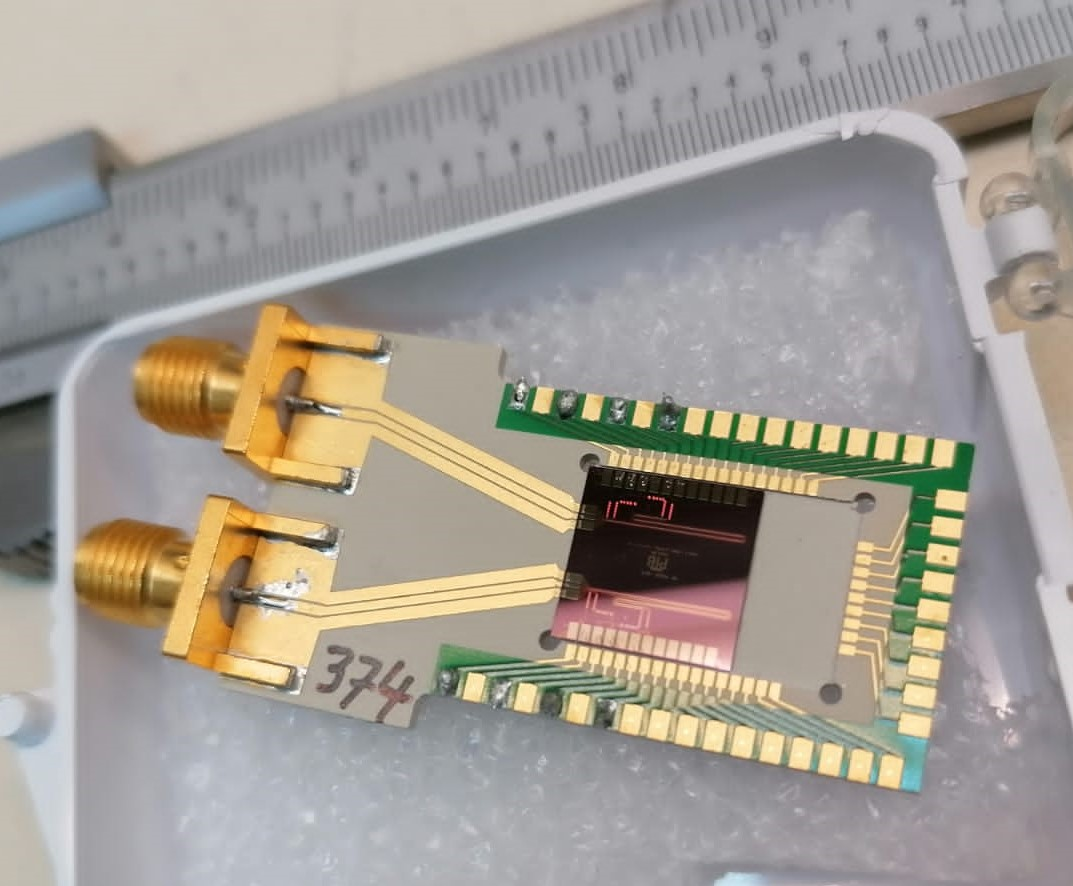
\includegraphics[width=0.75\linewidth]{figuras/jaws.jpg}
\caption{Chip JAWS construido en el PTB con 2 arrays de junturas Josephson disponible en el INTI}
\label{fig:chipJaws}
\end{figure}

Un esquema general de la futura construcción del sistema JAWS se muestra en la figura \ref{fig:esquemaJaws}. Lo que se hizo en este trabajo fue la generación numérica de los patrones de pulsos necesarios para cada señal que queramos generar.

\begin{figure}[H]
\centering
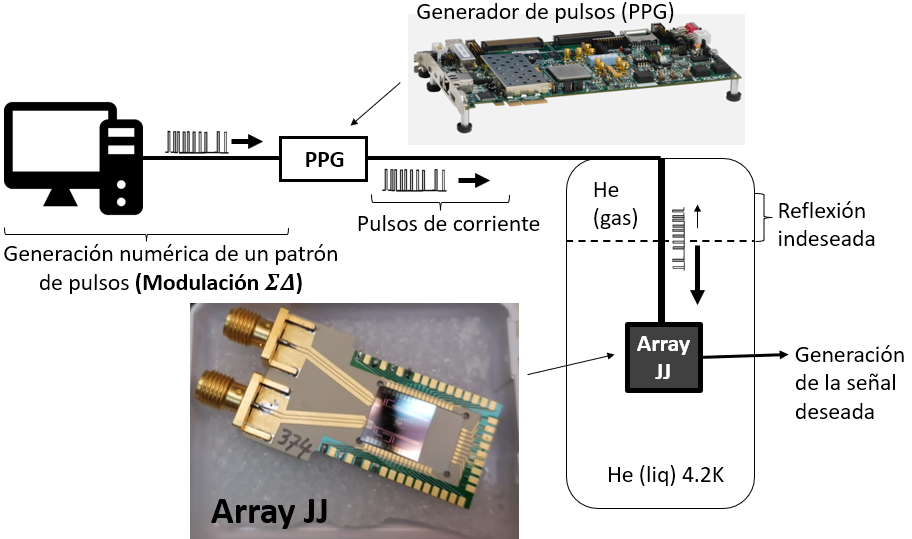
\includegraphics[width=\linewidth]{figuras/esquema_contruccion.png}
\caption{Esquema general de la construcción del sistema JAWS}
\label{fig:esquemaJaws}
\end{figure}
%El JAWS (Josephson Arbitrary Waveform Synthesizer) es el sintetizador de señales  más preciso que existe en la actualidad. Su operación consiste en mandar pulsos de corriente, en un rango de frecuencias de microondas, hacia un {\it array} de junturas de Josephson

Los patrones de pulsos generados siguen una técnica denominada modulación Sigma-Delta. La ventaja de este método particular es que tiene mucha fidelidad a la señal original, más precisamente: aumenta la relación señal a ruido. Aunque también hay que señalar que tiene algunas desventajas, como requerir mucho poder de cómputo frente a otras técnicas de conversión digital. Una comparación de algunas de estas técnicas se muestra en la figura \ref{fig:tecnicas}

\begin{figure}[H]
\centering
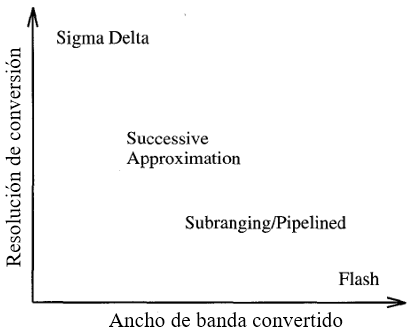
\includegraphics[width=0.75\linewidth]{figuras/fig3aziz.png}
\caption{Comparación de distintos métodos conversión digital. La modulación Sigma-Delta es una de ellas.}
\label{fig:tecnicas}
\end{figure}

La fidelidad a la señal consiste en limpiar el ruido presente en la zona de frecuencias de interés, y empujarlo hacia otras zonas del espectro, por lo general las altas frecuencias, para luego ser filtrado por un filtro pasabajos. Hay muchos tipos diferentes de modulación Sigma-Delta, como los que se centran en limpiar el ruido en una franja de frecuencia de interés (para luego pasar el filtro pasabanda correspondiente), pero no nos centramos en estos otros.
También existen optimizaciones, que lo que hacen es generar pulsos que tengan aún menos ruido, habiéndolo empujado más, pero esto es a costa del hardware del que se disponga.
Los pulsos generados por el algoritmo van a ser enviados a un generador de pulsos de corriente, FPGA (Field Programmable Gate Array) \cite{fpga}, en el cual se cargarán los pulsos de salida del script y generará la salida electrónica necesaria para el array de junturas Josephson. Las características de hardware del FPGA nos dirán qué modulaciones Sigma-Delta podremos usar, por ejemplo, no podremos usar ordenes $L$ elevados.



%%%%%

%Se usaron niveles de oversampling mucho menores para la simulacion, para poder visualizarse, ya que los niveles reales que se usaran seran del orden de OSR's de ~500



\subsection{Modulación $\Sigma\Delta$}

La modulación Sigma-Delta \cite{delarosa2011} \cite{aziz1996} es una técnica que permite representar una señal analógica a través de una señal digital de pocos valores. Intuitivamente, compensamos los pocos valores que podemos expresar digitalmente con una alta tasa de muestreo. Es una técnica muy conveniente para la construcción del JAWS, ya que tiene la particularidad de redistribuir el ruido no deseado hacia las altas frecuencias, lo que es ideal para el JAWS ya que el chip tiene impresos filtros pasabajos (figura \ref{fig:LPF}), de modo que el ruido final se reduce considerablemente.

\begin{figure}[H]
\centering
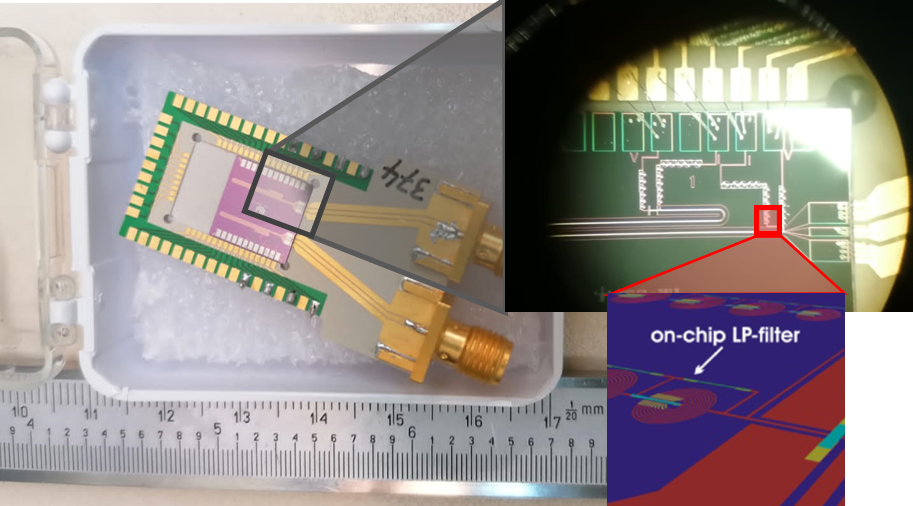
\includegraphics[width=\linewidth]{figuras/filtroLP.png}
\caption{Filtros pasabajos impresos en el chip JAWS del PTB}
\label{fig:LPF}
\end{figure}

La figura \ref{fig:LPF} muestra dos fotografías del chip del PTB actualmente presente en el INTI, junto a un gráfico sacado de la figura 24 del paper de Behr \cite{behr2012} mostrando el filtro pasabajos impreso en el chip.

%etimología? sumamos diferencias, promediamos la señal, pero sumamos(sigma) diferencias(delta)

Para el algoritmo, se parte de una señal temporal idealizada que llamamos $x(t)$, que representa la señal que queremos generar. Para ilustrar, supondremos que la señal es de tensión, aunque puede ser de unidades arbitrarias (u.a.). A lo largo de este trabajo, 1 u.a. representa al valor máximo que puede generar la salida del cuantizador, es decir, el generador de pulsos FPGA. A su vez, -1 u.a. es el valor negativo correspondiente.

A $x(t)$ se le realiza un muestreo temporal, i.e. quedarse con muestras de la misma a intervalos de tiempo iguales $T_s$, obteniendo una señal discretizada en el tiempo $x[n]$.

En procesamiento de señales, el teorema de Nyquist \cite{oppenheim} dice que para toda señal cuyo espectro de frecuencias esté contenido en una banda de frecuencias $[-f_B,+f_B]\subset \mathbb{R}$, con $f_B$ la menor frecuencia de muestreo tal que no se pierda ninugna información de la señal original es exactamente $f_N = 2 f_B$, y es la llamada frecuencia de Nyquist. A $f_B$ se la llama la frecuencia de banda, y es la mayor frecuencia que puede estar presente en la señal para que funcione el método.

El teorema de Nyquist asume que contamos con la posibilidad de generar cualquier señal en un rango contínuo que contenga a la señal original. Pero nosotros tenemos un generador de pulsos binarios, es decir, solo dos valores de tensión posibles: -1 y 1. Entonces, para poder llevar la información de la señal, vamos a tener que usar frecuencias de muestreo mucho mayores a $f_N$. Este proceso se llama oversampling. 

Se define el ratio de sobremuestreo OSR (oversampling ratio) como en la ecuación \ref{eq:OSR}, usando la misma definición que de la Rosa \cite{delarosa2011}. \footnote{Comparando con el paper de de la Rosa \cite{delarosa2011}, lo que ahí se llama $B_w$ nosotros lo llamamos $f_B$}

\begin{equation}
    \text{OSR} = \frac{f_s}{f_N} = \frac{f_s}{2 f_B}
    \label{eq:OSR}
\end{equation}

También definimos el ratio de muestreos por período $N_s$, exactamente como hace Benz en su paper de 1998 \cite{benz1998}, en la ecuación \ref{eq:ns}.

\begin{equation}
    N_s = f_s/f
    \label{eq:ns}
\end{equation}

La ecuación \ref{eq:ns} solo aplica cuando la señal de entrada es AC, y su frecuencia es $f$.

En la modulación sigma delta, es fundamental usar frecuencias de muestreo lo más altas posibles, ya que es de esta forma que se aumenta la precisión al solo contar con dos valores del generador de pulsos. Para llevar la información que lleva una señal que vive en un rango contínuo, usando solo dos valores discretos, se tiene que tener una gran cantidad de estos valores discretos por cada valor contínuo que queramos representar, y esta cantidad aumenta conforme aumentemos el valor de $f_s$. En nuestro caso, el generador tiene una $f_s = \SI{5}{\giga\hertz}$



Luego, se discretiza la tensión, lo que quiere decir que de todo el contínuo de tensiones, solo nos quedaremos con un conjunto finito de valores. En nuestro caso son 2, que definen los límites del rango de la señal que podremos generar.

En el apéndice y en la documentación del código se describe como se obtiene la modulación de orden L. Como ya mencionamos, limitaciones de hardware impedirán en la práctica realizar modulaciones con un orden $L$ elevado.


Al realizar la discretización en voltaje, lo que sucede es que estamos introduciendo un error, que llamamos ruido o error de cuantización $e_q$. Este error, en condiciones que son usuales en la práctica, puede ser modelado como ruido blanco, en otras palabras, como una variable aleatoria con función de distibución rectangular, entre los valores extremos del cuantizador. 
 
Asumiendo que el error es ruido blanco, el efecto producido por la modulación Sigma-Delta de orden $L\in\mathbb{N}$ es el aplicarle un filtro pasabajos con la forma funcional mostrada en la ecuación 
 
\begin{equation}
    NTF(z) = (1-z^-1)^L
    \label{eq:ntf}
\end{equation}

\begin{equation}
    z = e^{i2\pi f/f_s}
\end{equation}

Así, en la figura \ref{fig:NTF_spec} se muestra el efecto deseado de la modulación sobre el ruido de cuantización. El objetivo de esta modulación de pulsos particular es lograr que el ruido de cuantización se corra hacia lo más alto en frecuencias que nos sea posible. Mediante la modulación de orden L se logra que el ruido de cuantización se multiplique por una función moduladora llamada NTF (noise transfer function)

\begin{figure}[H]
\centering
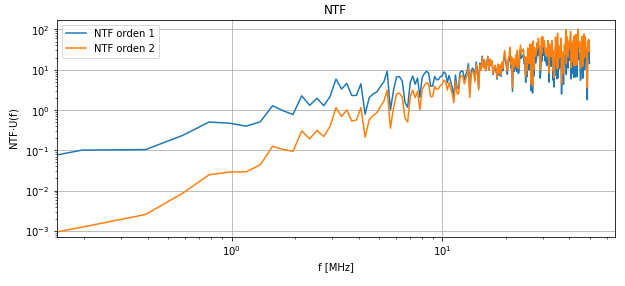
\includegraphics[width=\linewidth]{figuras/NTFs_espectro.png}
\caption{Comparación de los espectros de frecuencia de las NTF de orden 1 y 2}
\label{fig:NTF_spec}
\end{figure}

Para obtener lo observado en la figura \ref{fig:NTF_spec}, se modeló el ruido de cuantización como una variable aleatoria de dsitribución uniforme entre los valores del cuantizador, i.e. ruido blanco. Haciendo una transformada rápida de Fourier (FFT) de este ruido, se obtiene también ruido blanco, y este espectro es modulado por el valor absoluto de la NTF, que es lo que se observa en la figura \ref{fig:NTF_spec}. En particular, se observa que la modulación de orden 2 es más efectiva al trasladar más ruido desde las bajas hacia las altas frecuencias. 
Es importante notar que esto es solo un modelo teórico, dado que en realidad $e_q$ no es una variable aleatoria. Pero más adelante (ver figura \ref{fig:espectro}) se va a confirmar que el ruido de la señal generada se corre conforme indica la NTF.


\section{Descripción de la simulación numérica}


El código utilizado genera distintas variables presentes en la modulación sigma delta, y permite hacer un análisis muy detallado a partir de las mismas. En la figura \ref{fig:bloques} se muestra el diagrama de bloques representativo del algoritmo de modulación de 1er orden \cite{script}.

\begin{figure}[H]
\centering
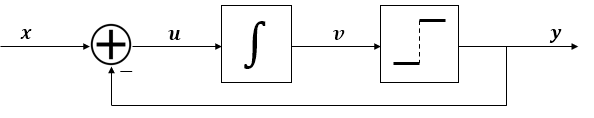
\includegraphics[width=\linewidth]{figuras/bloques_1erorden.png}
\caption{Diagrama de bloques correspondiente a la modulación $\Sigma\Delta$ de 1er orden}
\label{fig:bloques}
\end{figure}

En el apéndice se describe muy brevemente como se leen estos diagramas, y como se pueden traducir a un método iterativo en las 4 variables presentes: $x,u,v,y$.
La primera, $x$, representa la señal analógica de entrada, que es la señal que queremos generar. $u$ y $v$ son variables auxiliares, en donde $v$ es la integral de $u$, y $u$ es la diferencia $x-y$. $y$ es la salida final del cuantizador, que tiene en nuestro caso solo 2 valores posibles.


En este trabajo se implementó, siguiendo diferentes publicaciones (\cite{delarosa2011}, \cite{aziz1996}), el algoritmo de modulación Sigma-Delta de 1er orden en Python. Esto permitió explorar diferentes aspectos del método que no eran muy accesibles desde otras implementaciones, de manera muy sencilla.
Las implementaciones anteriores contienen optimizaciones adicionales que por el momento nuestro código no incluye. La más conocida es el paquete de Matlab de Richard Scherier \cite{DSmatlab}, sobre la cual se basa el paquete de Python de G. Venturini \cite{DSpython}. %Este último paquete fue usado para contrastar cualitativamente los pulsos generados por nuestro código, además de los resultados obtenidos en simulaciones numéricas de distintas fuentes \cite{aziz1996}, \cite{delarosa2011}.

En la figura \ref{fig:integrador} se muestra mejor el comportamiento de las variables $u$ y $v$ para cuando se quiere generar una señal DC de valor 0.8 u.a. Se observa que hay un período en el que la señal $u=x-y$ es ligeramente negativa, esto es porque $x=0.8$ es ligeramente inferior al nivel superior $y=1$ (todo en unidades arbitrarias). Durante este período, se van sumando estos valores de $u$ al valor de $v$, que en la figura \ref{fig:integrador} es la pendiente negativa que está en el área de integración negativa, sombreada en azul.


\begin{figure}[H]
\centering
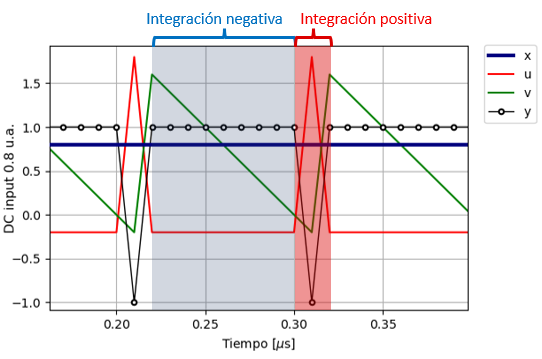
\includegraphics[width=\linewidth]{figuras/integracion.png}
\caption{Ejemplo del funcionamiento del integrador en la modulación a 1er orden}
\label{fig:integrador}
\end{figure}

Llega un punto en que $v$ pasa a ser negativo, de modo que, al pasar al cuantizador, generará un pulso $y$ negativo, luego de varios positivos. Esto es lo que se ve en el área de integración positiva: el valor de $u$, en ese lapso muy corto de tiempo, es positivo y muy grande, de tal manera que basta solo uno para volver al régimen de pulsos positivos. De esta manera el algoritmo genera la proporción de pulsos negativos y positivos deseada.



\section{Descripción del experimento}



\section{Resultados y Análisis}

Usando nuestro script \cite{script}, generamos los pulsos correspondientes a una señal DC para reproducir los resultados que se muestran en \cite{aziz1996}. En la figura 







\newpage 
\bibliographystyle{unsrt}
\bibliography{references}


\nocite{*} % Insert publications even if they are not cited in the poster

\end{multicols}

\end{document}
